%% LaTeX2e class for student theses
%% sections/apendix.tex
%% 
%% Karlsruhe Institute of Technology
%% Institute of Information Security and Dependability
%% Software Design and Quality (SDQ)
%%
%% Dr.-Ing. Erik Burger
%% burger@kit.edu
%%
%% Version 1.5, 2024-02-12

\iflanguage{english}
{\chapter{Appendix}}    % english style
{\chapter{Anhang}}      % german style
\label{chap:appendix}

\lstset{
  basicstyle=\ttfamily\small,
  frame=single,
  breaklines=true,      
  breakatwhitespace=true,
  breakindent=0em,
  breakautoindent=true,
}

%% -------------------
%% | Example content |
%% -------------------
\section{Prompts}
\label{sec:appendix:prompts}

\setcounter{figure}{0}

\subsection{HubLink}
\label{sec:appendix:hublink_prompts}

\begin{lstlisting}[caption={Partial Answer Generation Prompt}]
### Task Description:
  You are given a question and a set of context passages. Your task is:
  1. Carefully examine the provided contexts.
  2. Extract all explicitly stated information from the contexts that helps answer the question (even if the information is partial, incomplete, or does not fully resolve the question).
  2. If you find relevant but partial information, you must clearly present it.
  3. ONLY IF no explicitly relevant information at all is present, then clearly state:
  ```
  Insufficient Information.
  ```
  ### Examples:
  #### Example 1: No Relevant Information
  - **Question:** "Who wrote Paper X?"
  - **Provided Texts:**  
    "Paper X discusses software design."
  - **Answer:**  
    ```
    Insufficient information.
    ```
  #### Example 2: Direct Information
  - **Question:** "When was Paper X published?"
  - **Provided Texts:**  
    "Paper X was published in 2020."
  - **Answer:**  
    "Paper X was published in 2020."
  #### Example 3: Partial Information
  - **Question:** "When was Paper Y published compared to Paper Z?"
  - **Provided Texts:**  
    "Paper Y was published in 2018."
  - **Answer:**  
    "Paper Y was published in 2018. However, the publication date of Paper Z is not provided in the texts. "
  #### Example 4: Partial Information
  - **Question:** "How many papers include X?"
  - **Provided Texts:**  
    "Paper A includes X."
  - **Answer:**  
    "The Paper with the title 'Paper A' includes X. However, this is only one instance, and there may be more papers that include X."
  ---
  ### Start Your Task
  If any relevant information is found, even if it is just a single mention or a partial detail, forward that information. Do not conclude 'Insufficient Information' if at least one explicit data point exists.
  **Question:**
  {question}
  **All Texts have the following information in common:**
  {common_information}
  **Provided Texts:**
  {texts}
  **Answer:**
\end{lstlisting}


\begin{lstlisting}[caption={Final Answer Generation Prompt}]
  ### Task Description:
  You are an expert text synthesizer. Your task is to combine the provided partial answers into a coherent and comprehensive final answer. Each partial answer has a source identification provided as [ID] that you should cite in the final answer. 

  ### Constraints:

  - Do **not** introduce any external information, personal opinions, or interpretations beyond what is provided in the partial answers.
  - If a partial answer contains identification objects such as object_1, object_2, etc., do not include the object identification in the final aswer just use the source id [ID] as mentioned above.
  - Ensure clarity and coherence in the final output.
  
  ### Question:
  {question}

  ### Partial Answers:
  {partial_answers}
  
  ### Final Answer:
\end{lstlisting}

\begin{lstlisting}[caption={Question Component Extraction Prompt}]
  ### Task Description:
  Please analyze the following question and break it down into its key components or claims. 

  ### Instructions:
  - Break down the question into its key components or claims.
  - Your output has to be a valid python list of strings.
  - Do not use any external information, personal opinions, or interpretations beyond the given texts. Do not make any assumptions and do not answer the question.
  - Do not include any additional explanations or commentary. Just provide the list of components.

  ### Examples:
  Question: What are the research questions in the paper titled 'Artificial Intelligence in Healthcare'?
  Components: ['Research Questions', 'Artificial Intelligence in Healthcare']
  Question: Which publications include the research object 'Architecture Analysis Method'?
  Components: ['Research Object', 'Architecture Analysis Method']
  Question: Which papers have been published by SpringerLink in 2020?
  Components: ['Publisher', 'SpringerLink', '2020']

  ### Start Your Task:
  Question: {question}
\end{lstlisting}

\begin{lstlisting}[caption={Triple Filtering Prompt}]
  ### Task Description:
  You are a knowledgeable assistant. Given a question, a answer and a list of ID-triple mappings in the format "ID: (subject, predicate, object)" determine which triples provide direct information essential for answering the question. If a triple is relevant or partially relevant, include its ID in the final output; otherwise, exclude it. Provide in your answer only a list of the final triple IDs and do not provide any additional explanations or commentary. If no triples are relevant, return an empty list.

  ### Required Output Format:
  [ID1, ID2, ID3, ...]

  ### Question:
  {question}

  ### Answer:
  {answer}

  ### Retrieved Contexts:
  {contexts}
\end{lstlisting}



\subsection{Question Augmentation and Reranking}

\begin{lstlisting}[caption={Question Augmentation Prompt},label={lst:question_augmentation_prompt}]
You are an assistant designed to enhance user questions to improve the effectiveness of a Retrieval-Augmented Generation (RAG) system. Your task is to augment the original question by clarifying ambiguities, incorporating related keywords or phrases that will help the retrieval system fetch more accurate and comprehensive information, and add nouns or noun phrases to terms to clearly indicate their types or roles.

**Guidelines:**
1. **Clarify Ambiguous Terms:** If the original question contains terms that could be interpreted in multiple ways, clarify their meanings based on common usage or provide additional context.
2. **Incorporate Related Keywords:** Add synonyms or related terms that are pertinent to the topic to broaden the retrieval scope without deviating from the original intent.
3. **Explicit Noun Phrases:** Incorporate nouns or noun phrases to terms to specify their types (e.g., author, year, title, person, etc.)
4. **Maintain Original Intent:** Ensure that the augmented question retains the original purpose and does not introduce unrelated elements.

**Format:**
Provide the augmented question directly without additional commentary.

**Original Question:** "{original_question}"
\end{lstlisting}

\begin{lstlisting}[caption={Context Reranking Prompt},label={lst:context_reranking_prompt}]
You are an intelligent assistant specialized in information retrieval and ranking.

Given a user question and a list of retrieved context IDs mapped to their respective contexts, your task is to rerank the context IDs in order of their relevance to the question. The structure of the mapping is 'ID: context'. The most relevant context ID should be listed first, followed by the next most relevant, and so on.
Think in steps: First determine the most important entity that is asked for in the question, then check which contexts are the most relevant to that entity. Then continue to the next most important entity and so on.

Provide only the "Re-Ranked Context IDs" for example: [2, 5, 8] without any additional explanations or commentary.

**Question:**
{question}

**Retrieved Contexts:**
{contexts}

**Instructions:**
- Analyze each context in relation to the question.
- Determine the relevance of each context to answering the question.
- Rank the context IDs from most relevant (1) to least relevant (n).

**Re-Ranked Contexts:**
\end{lstlisting}

\begin{lstlisting}[caption={Answer Generation Prompt},label={lst:answer_generation_prompt}]
You are an advanced AI language model tasked with answering questions based solely on the provided context.
Your responses must be accurate, concise, and derived exclusively from the given information.

## Context Explanation:
{context_explanation}

## Context:
{context}

## Question:
{question}

## Instructions:
1. Carefully analyze the provided context.
2. Formulate a clear and concise answer based exclusively on the given context.
3. If the context lacks sufficient information to answer the question fully:
a. Provide any partial information that is relevant and available.
b. Clearly state: "The question cannot be fully answered with the provided context."
4. Do not introduce any external information or make assumptions beyond the given context.
5. If dealing with vector store chunks, try to connect information across chunks when relevant.
6. For knowledge graph data, interpret the relationships between entities to derive your answer.
7. Maintain a confident tone, but also indicate any uncertainties that arise from limitations in the context.

## Answer:
\end{lstlisting}

\section{ORKG Contribution Templates}
\label{sec:appendix:orkg_contribution_templates}

\begin{figure}[H]
    \centering
    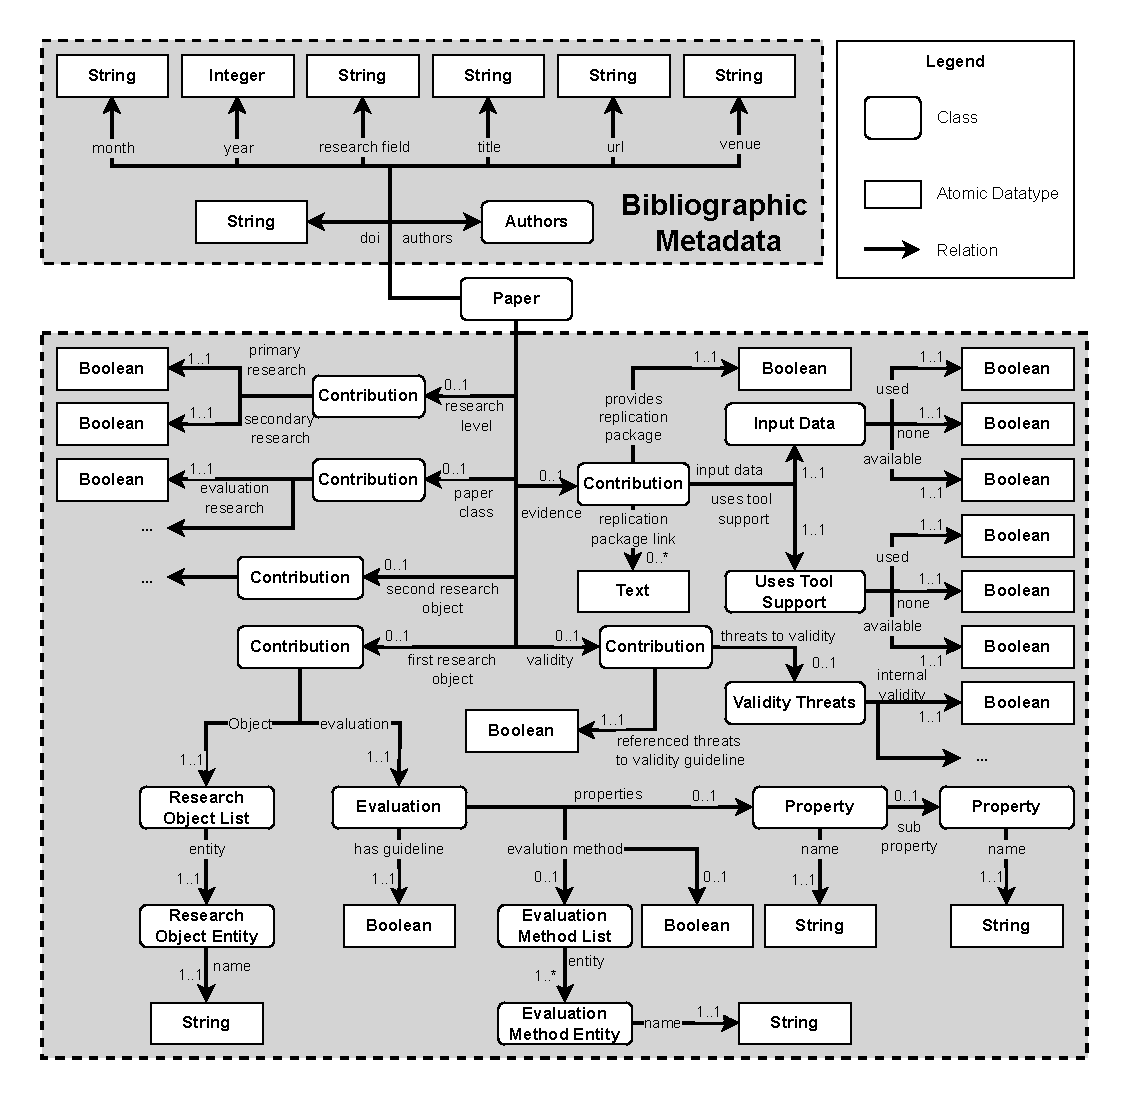
\includegraphics[width=0.90\linewidth]{figures/orkg/template_overview-deep_distributed.drawio.pdf}
    \caption[Template for First Graph Variant]{Template for the \textbf{GV1} graph variant which stores data deep and distributed.}
\end{figure}

\begin{figure}[H]
    \centering
    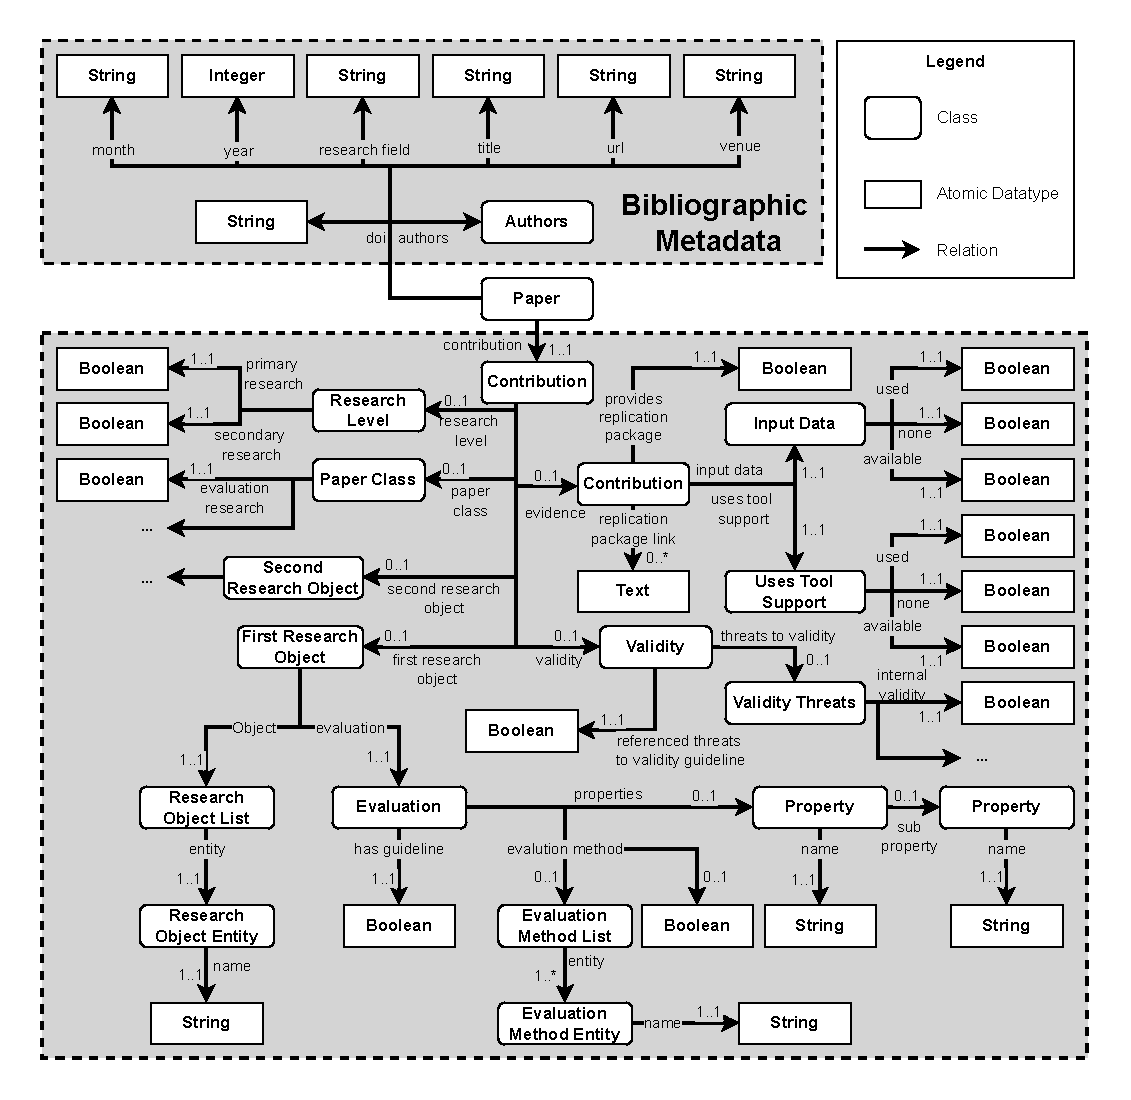
\includegraphics[width=0.90\linewidth]{figures/orkg/template_overview-deep_centralized.drawio.pdf}
    \caption[Template for Second Graph Variant]{Template for the \textbf{GV2} graph variant which stores data deep and centralized.}
\end{figure}

\begin{figure}[H]
    \centering
    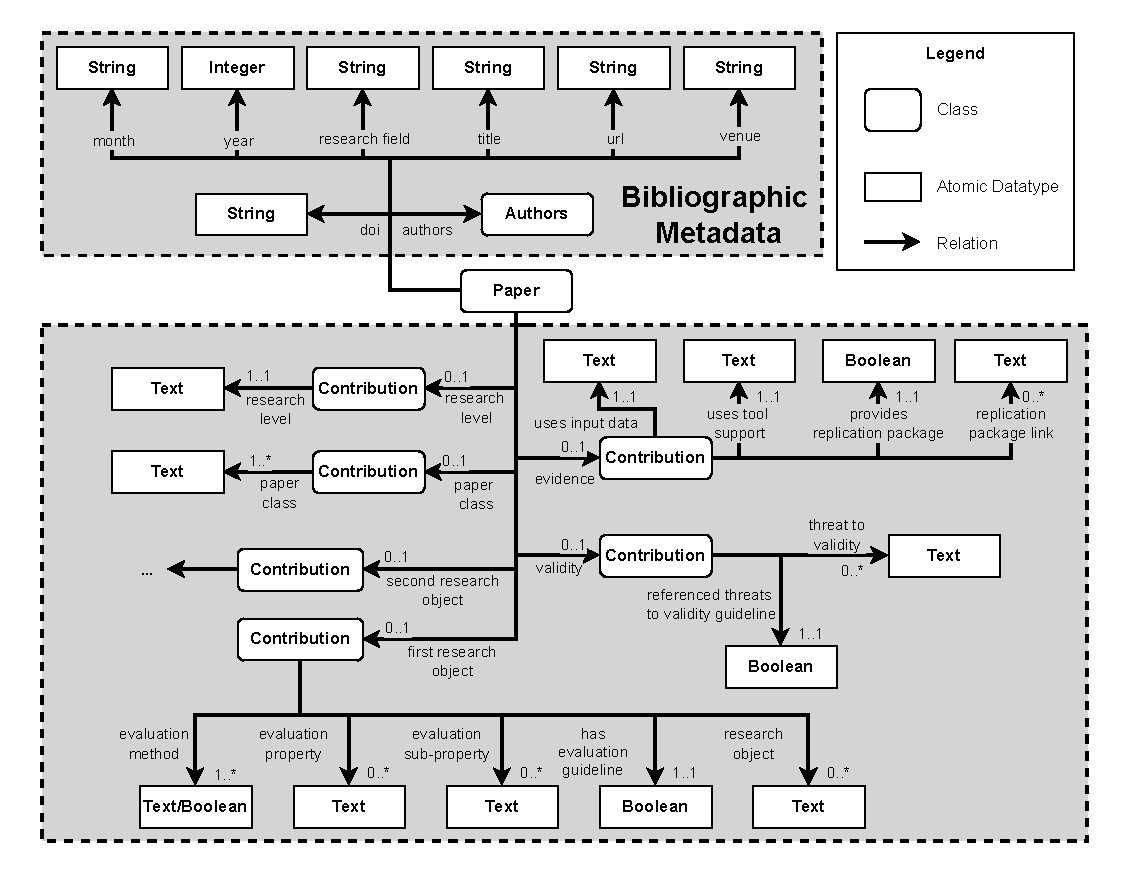
\includegraphics[width=0.90\linewidth]{figures/orkg/template_overview-flat_distributed.drawio.pdf}
    \caption[Template for Third Graph Variant]{Template for the \textbf{GV3} graph variant which stores data flat and distributed.}
\end{figure}

\begin{figure}[H]
    \centering
    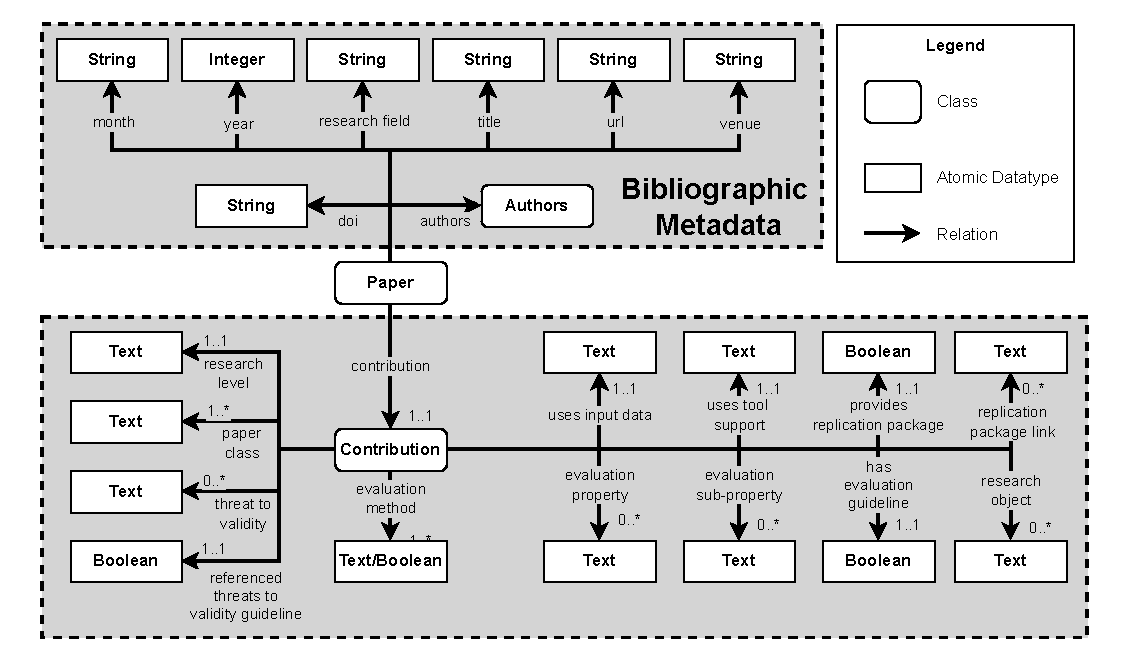
\includegraphics[width=0.90\linewidth]{figures/orkg/template_overview-flat_centralized.drawio.pdf}
    \caption[Template for Fourth Graph Variant]{Template for the \textbf{GV4} graph variant which stores data flat and centralized.}
\end{figure}


\section{Additional Evaluation Results}
\label{sec:appendix:additioal_evaluation_results}

\subsection{Additional Evaluation Results for Operation Complexity}
\label{sec:appendix:additional_evaluation_results_operation_complexity}

\begin{table}[H]
\centering
\resizebox{\textwidth}{!}{%
\begin{tabular}{@{}llllllll@{}}
\toprule
Retrieval Operation & Recall & Precision & F1 & Hits@10 & Map@10 & MRR@10 & EM@10 \\ 
\midrule
\multicolumn{8}{c}{DiFaR} \\
\midrule
basic & 0.528 & 0.006 & 0.006 & 0.167 & 0.083 & 0.083 & 0.017 \\
aggregation & 0.365 & 0.008 & 0.017 & 0.236 & 0.199 & 0.302 & 0.083 \\
counting & 0.350 & 0.007 & 0.017 & 0.257 & 0.215 & 0.267 & 0.092 \\
ranking & 0.164 & 0.005 & 0.013 & 0.111 & 0.089 & 0.190 & 0.058 \\
comparative & 0.363 & 0.014 & 0.029 & 0.247 & 0.130 & 0.331 & 0.154 \\
relationship & 0.380 & 0.017 & 0.032 & 0.270 & 0.239 & 0.545 & 0.196 \\
negation & 0.364 & 0.013 & 0.031 & 0.219 & 0.107 & 0.308 & 0.131 \\
superlative & 0.346 & 0.018 & 0.034 & 0.113 & 0.087 & 0.278 & 0.075 \\
\midrule
\multicolumn{8}{c}{Mindmap} \\
\midrule
basic & 0.278 & 0.020 & 0.037 & 0.056 & 0.006 & 0.006 & 0.006 \\
aggregation & 0.115 & 0.031 & 0.046 & 0.004 & 0.000 & 0.004 & 0.004 \\
counting & 0.182 & 0.041 & 0.065 & 0.004 & 0.000 & 0.004 & 0.004 \\
ranking & 0.105 & 0.029 & 0.043 & 0.016 & 0.002 & 0.009 & 0.008 \\
comparative & 0.026 & 0.010 & 0.014 & 0.005 & 0.005 & 0.042 & 0.004 \\
relationship & 0.116 & 0.055 & 0.073 & 0.018 & 0.002 & 0.015 & 0.013 \\
negation & 0.054 & 0.020 & 0.029 & 0.023 & 0.003 & 0.023 & 0.019 \\
superlative & 0.079 & 0.030 & 0.041 & 0.000 & 0.000 & 0.000 & 0.000 \\
\midrule
\multicolumn{8}{c}{FiDeLiS} \\
\midrule
basic & 0.333 & 0.208 & 0.245 & 0.333 & 0.306 & 0.306 & 0.220 \\
aggregation & 0.035 & 0.016 & 0.022 & 0.035 & 0.013 & 0.028 & 0.017 \\
counting & 0.021 & 0.012 & 0.015 & 0.021 & 0.010 & 0.021 & 0.012 \\
ranking & 0.102 & 0.037 & 0.051 & 0.101 & 0.038 & 0.072 & 0.029 \\
comparative & 0.157 & 0.067 & 0.087 & 0.157 & 0.099 & 0.173 & 0.079 \\
relationship & 0.052 & 0.044 & 0.048 & 0.053 & 0.033 & 0.121 & 0.046 \\
negation & 0.011 & 0.011 & 0.011 & 0.010 & 0.010 & 0.062 & 0.006 \\
superlative & 0.045 & 0.047 & 0.045 & 0.045 & 0.019 & 0.062 & 0.031 \\
\bottomrule
\end{tabular}%
}
\caption[Baseline Performance by Operation Complexity]{Impact of the retrieval operation on the performance of the \gls{kgqa} baseline approaches. The results are based on graph variant \hyperref[enum:gv1]{\textbf{GV1}} and all metrics have been macro averaged.}
\label{tab:baseline_performance_operation_complexity}
\end{table}

\subsection{Additional Evaluation Results for Use Cases}
\label{sec:appendix:additional_evaluation_results_use_cases}

\begin{table}[H]
\centering
% \resizebox{\textwidth}{!}{%
\begin{tabular}{@{}llllllll@{}}
\toprule
Use Case & Recall & Precision & F1 & Hits@10 & Map@10 & MRR@10 & EM@10 \\ 
\midrule
\multicolumn{8}{c}{DiFaR} \\
\midrule
1 & 0.588 & 0.010 & 0.021 & 0.436 & 0.352 & 0.538 & 0.129 \\ 
2 & 0.104 & 0.001 & 0.001 & 0.000 & 0.000 & 0.000 & 0.000 \\ 
3 & 0.453 & 0.016 & 0.032 & 0.302 & 0.238 & 0.412 & 0.156 \\ 
4 & 0.264 & 0.011 & 0.021 & 0.191 & 0.145 & 0.324 & 0.121 \\ 
5 & 0.275 & 0.009 & 0.020 & 0.070 & 0.029 & 0.101 & 0.048 \\ 
6 & 0.421 & 0.014 & 0.031 & 0.255 & 0.152 & 0.400 & 0.155 \\ 
\midrule
\multicolumn{8}{c}{Mindmap} \\
\midrule
1 & 0.177 & 0.034 & 0.053 & 0.005 & 0.001 & 0.006 & 0.004 \\ 
2 & 0.023 & 0.014 & 0.017 & 0.000 & 0.000 & 0.000 & 0.000 \\ 
3 & 0.208 & 0.033 & 0.054 & 0.035 & 0.004 & 0.007 & 0.007 \\ 
4 & 0.121 & 0.043 & 0.061 & 0.022 & 0.002 & 0.015 & 0.014 \\ 
5 & 0.098 & 0.034 & 0.048 & 0.016 & 0.005 & 0.041 & 0.012 \\ 
6 & 0.072 & 0.020 & 0.030 & 0.004 & 0.000 & 0.003 & 0.003 \\ 
\midrule
\multicolumn{8}{c}{FiDeLiS} \\
\midrule
1 & 0.269 & 0.253 & 0.271 & 0.148 & 0.268 & 0.183 & 0.182 \\ 
2 & 0.125 & 0.043 & 0.065 & 0.036 & 0.125 & 0.055 & 0.025 \\ 
3 & 0.057 & 0.036 & 0.060 & 0.052 & 0.057 & 0.052 & 0.047 \\ 
4 & 0.061 & 0.036 & 0.150 & 0.053 & 0.061 & 0.056 & 0.043 \\ 
5 & 0.040 & 0.018 & 0.033 & 0.014 & 0.041 & 0.020 & 0.012 \\ 
6 & 0.047 & 0.025 & 0.076 & 0.030 & 0.047 & 0.035 & 0.031 \\ 
\bottomrule
\end{tabular}%
% }
\caption[Baseline Performance by Use Case]{Assessment of different scholarly use cases on the retrieval performance for the baseline \gls{kgqa} approaches. The results are based on graph variant \hyperref[enum:gv1]{\textbf{GV1}} and all metrics have been macro averaged. The use cases are introduced in Section~\ref{sec:qa_use_cases}.}
\label{tab:baseline_performance_use_case}
\end{table}



\subsection{Additional Evaluation Results for Type Information in the Question}
\label{sec:appendix:additional_evaluation_results_type_information}

\begin{table}[H]
\centering
% \resizebox{\textwidth}{!}{%
\begin{tabular}{@{}llllllll@{}}
\toprule
Semi-Typed & Recall & Precision & F1 & Hits@10 & Map@10 & MRR@10 & EM@10 \\ 
\midrule
\multicolumn{8}{c}{DiFaR} \\
\midrule
True & 0.256 & 0.189 & 0.349 & 0.011 & 0.359 & 0.023 & 0.128 \\ 
False & 0.155 & 0.109 & 0.238 & 0.010 & 0.343 & 0.021 & 0.078 \\ 
\midrule
\multicolumn{8}{c}{Mindmap} \\
\midrule
True & 0.006 & 0.001 & 0.006 & 0.029 & 0.105 & 0.042 & 0.005 \\ 
False & 0.024 & 0.004 & 0.021 & 0.031 & 0.133 & 0.047 & 0.010 \\ 
\midrule
\multicolumn{8}{c}{FiDeLiS} \\
\midrule
True & 0.108 & 0.076 & 0.121 & 0.065 & 0.108 & 0.076 & 0.062 \\ 
False & 0.075 & 0.048 & 0.083 & 0.039 & 0.075 & 0.049 & 0.043 \\ 
\bottomrule
\end{tabular}%
% }
\caption[Results for Baselines on Semi-Typed Questions]{The impact of questions that add information about the condition types compared to those that do not for the baseline \gls{kgqa} approaches. The results are based on graph variant \hyperref[enum:gv1]{\textbf{GV1}} and all metrics have been macro averaged.}
\label{tab:baseline_performance_semi_typed}
\end{table}